% Source: graduate-coursework/Research/Intro_to_Agents/handouts/Part6_MultiTier_Architecture.tex

\documentclass[border=4pt]{standalone}
\usepackage{amsmath,amssymb,amsfonts}
\usepackage[T1]{fontenc}
\usepackage{graphicx}
\usepackage{lmodern}
\usepackage{tikz}
\usepackage{xcolor}
\usetikzlibrary{shapes,arrows.meta,positioning,calc,fit,backgrounds,chains,decorations.pathreplacing}

\definecolor{UofSCGarnet}{HTML}{73000a}
\definecolor{UofSCBlack}{HTML}{000000}
\definecolor{UofSCWhite}{HTML}{ffffff}
\definecolor{UofSCRose}{HTML}{CC2E40}
\definecolor{UofSCAtlantic}{HTML}{466A9F}
\definecolor{UofSCCongaree}{HTML}{1F414D}
\definecolor{UofSCHorseshoe}{HTML}{65780B}
\definecolor{UofSCGrass}{HTML}{CED318}
\definecolor{UofSCHoneycomb}{HTML}{A49137}
\definecolor{UofSC90Black}{HTML}{363636}
\definecolor{UofSC70Black}{HTML}{5C5C5C}
\definecolor{UofSC50Black}{HTML}{A2A2A2}
\definecolor{UofSCWarmGrey}{HTML}{676156}
\definecolor{UofSCSandstorm}{HTML}{FFF2E3}
\definecolor{UofSCDarkGarnet}{HTML}{570008}
\definecolor{UofSCAzalea}{HTML}{844247}

\tikzset{
    % Base node style
    basenode/.style={
        draw=UofSCBlack,
        fill=UofSCWhite,
        line width=0.8pt,
        minimum height=0.8cm,
        minimum width=2cm,
        align=center,
        font=\small
    },
    % Strategy layer style
    strategynode/.style={
        basenode,
        fill=UofSCGarnet,
        text=UofSCWhite,
        minimum height=1cm,
        minimum width=4cm
    },
    % Planning layer style
    planningnode/.style={
        basenode,
        fill=UofSCAtlantic,
        text=UofSCWhite,
        minimum height=0.9cm,
        minimum width=3.5cm
    },
    % Execution layer style
    execnode/.style={
        basenode,
        fill=UofSCCongaree,
        text=UofSCWhite,
        minimum height=0.8cm,
        minimum width=2.5cm
    },
    % Generic box
    genericbox/.style={
        basenode,
        minimum width=2.8cm
    },
    % Arrow styles (straight lines only)
    myarrow/.style={
        ->,
        >=Stealth,
        line width=0.8pt,
        draw=UofSCBlack
    },
    % Bidirectional arrow
    biarrow/.style={
        <->,
        >=Stealth,
        line width=0.8pt,
        draw=UofSCBlack
    },
    % Phase box style
    phasebox/.style={
        basenode,
        minimum width=3.5cm,
        minimum height=1.2cm,
        font=\small\bfseries
    },
    % Small box
    smallbox/.style={
        basenode,
        minimum width=1.5cm,
        minimum height=0.6cm,
        font=\scriptsize
    },
    % Leader node
    leadernode/.style={
        basenode,
        fill=UofSCGarnet,
        text=UofSCWhite,
        minimum width=3cm,
        minimum height=1cm
    },
    % Worker node
    workernode/.style={
        basenode,
        fill=UofSC70Black,
        text=UofSCWhite,
        minimum width=1.2cm,
        minimum height=0.7cm,
        font=\scriptsize
    }
}

\begin{document}
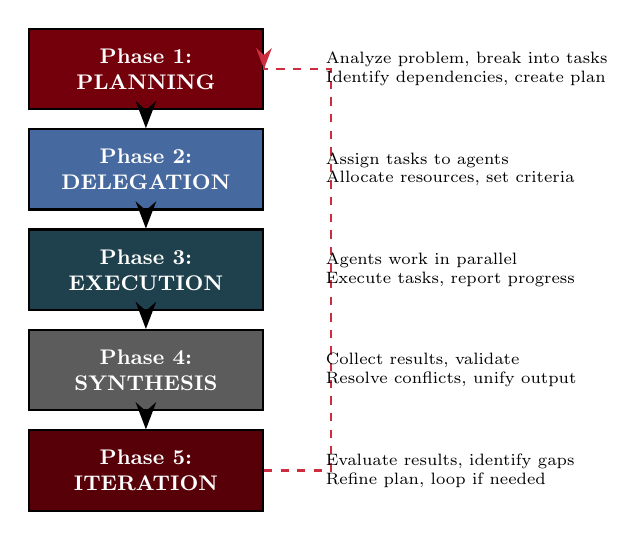
\begin{tikzpicture}[scale=0.85, transform shape]
        % Phase boxes
        \node[phasebox, fill=UofSCGarnet, text=white] (p1) at (0,5) {Phase 1:\\PLANNING};
        \node[phasebox, fill=UofSCAtlantic, text=white] (p2) at (0,3.5) {Phase 2:\\DELEGATION};
        \node[phasebox, fill=UofSCCongaree, text=white] (p3) at (0,2) {Phase 3:\\EXECUTION};
        \node[phasebox, fill=UofSC70Black, text=white] (p4) at (0,0.5) {Phase 4:\\SYNTHESIS};
        \node[phasebox, fill=UofSCDarkGarnet, text=white] (p5) at (0,-1) {Phase 5:\\ITERATION};

        % Arrows
        \draw[myarrow, line width=1.5pt] (p1) -- (p2);
        \draw[myarrow, line width=1.5pt] (p2) -- (p3);
        \draw[myarrow, line width=1.5pt] (p3) -- (p4);
        \draw[myarrow, line width=1.5pt] (p4) -- (p5);

        % Feedback loop
        \draw[myarrow, line width=1pt, dashed, color=UofSCRose] (p5.east) -- ++(1,0) -- ++(0,6) -- ++(-1,0) -- (p1.east);

        % Descriptions
        \node[font=\scriptsize, align=left, right=0.8cm of p1] {Analyze problem, break into tasks\\Identify dependencies, create plan};
        \node[font=\scriptsize, align=left, right=0.8cm of p2] {Assign tasks to agents\\Allocate resources, set criteria};
        \node[font=\scriptsize, align=left, right=0.8cm of p3] {Agents work in parallel\\Execute tasks, report progress};
        \node[font=\scriptsize, align=left, right=0.8cm of p4] {Collect results, validate\\Resolve conflicts, unify output};
        \node[font=\scriptsize, align=left, right=0.8cm of p5] {Evaluate results, identify gaps\\Refine plan, loop if needed};
    \end{tikzpicture}
\end{document}
